%% Created by M.Sc. Nils Lutz
%%    For questions, comments, suggestions etc. send an email to:
%%    info@nilslutz.de
%%
%% Version: September 17, 2019
%%
%% Note: Has only been tested with pdflatex, not latex (dvi). Still, there is
%% theoretical support also for latex.
%%
\documentclass[enabledeprecatedfontcommands,12pt,bibtotoc]{scrartcl}

%% packages
\usepackage[T1]{fontenc}
\usepackage[utf8]{inputenc}       % Standard for Linux
\usepackage{lmodern}
%\usepackage[latin1]{inputenc}    % Standard for Windows
\usepackage{ngerman}              % For German language
\usepackage{fancyhdr}
\usepackage{geometry}
\usepackage{ifpdf}
\usepackage{setspace}             % For line spread
\usepackage[printonlyused, withpage, smaller]{acronym}
\usepackage[authoryear, round, sort]{natbib}
\usepackage{csquotes}
\renewcommand{\mkbegdispquote}[2]{\itshape}
\usepackage{enumitem}
\usepackage{tabularx}
\usepackage{booktabs}
\usepackage{lscape}
\usepackage[table,xcdraw]{xcolor}
\usepackage{color}
\usepackage{float}
\usepackage{nicefrac}
\usepackage{listings} %For code in appendix
\usepackage{textcomp} % for upquote
\usepackage{blindtext}

\lstset
{ %Formatting for code in appendix
  backgroundcolor=\color{white},
  basicstyle=\ttfamily\footnotesize,
  breakatwhitespace=false,
  breaklines=true,
  captionpos=b,
  columns=fullflexible,
  commentstyle=\color{mediumgray}\upshape,
  emph={},
  emphstyle=\color{crimson},
  extendedchars=true,  % requires inputenc
  fontadjust=true,
  identifierstyle=\color{black},
  keepspaces=true,
  keywordstyle=\color{mediumblue},
  keywordstyle={[2]\color{darkviolet}},
  keywordstyle={[3]\color{royalblue}},
  numbers=left,
  numbersep=5pt,
  numberstyle=\tiny\color{black},
  rulecolor=\color{black},
  showlines=true,
  showspaces=false,
  showstringspaces=false,
  showtabs=false,
  stringstyle=\color{forestgreen},
  tabsize=1,
  title=\lstname,
  upquote=true  % requires textcomp
}

% For pdflatex
\ifpdf
  % One of these two:
  \usepackage[pdftex]{graphicx}
  %\usepackage[pdftex]{epsfig}

  \usepackage[pdftex]{hyperref}
% For latex (dvi)
\else
  % One of these two:
  \usepackage[dvips]{graphicx}
  %\usepackage[dvips]{epsfig}

  % make the command \href from hyperref available as a 'print only'
  \newcommand{\href}[2]{#2}
\fi

%% Picture options
\graphicspath{{pictures/}}         % Default path to pictures used
\DeclareGraphicsExtensions{.png}   % More extensions can be added

% Hyper ref coloring
\hypersetup{colorlinks, citecolor=black, linkcolor= black, urlcolor=black}

%% Pagestyle options
\pagestyle{fancy}
%\lhead{}
%\chead{}
%\rhead{}
%\lfoot{Daniel Süpke}
%\cfoot{}
%\rfoot{}
\renewcommand{\headrulewidth}{0.4pt}

\geometry{a4paper,left=3cm,right=3cm}
%\geometry{a4paper,left=3cm,right=2.5cm}   % Please use these settings for a PhD-thesis

%% Document start
\begin{document}

\pagenumbering{Roman}

% Insert titlepage
%% Title page
\begin{titlepage}
  \begin{centering}
  \begin{figure}[h!]
    \centering
    
\includegraphics[width=310pt]{Jade_Logo}
  \end{figure}

  %\vspace*{-0.8cm}

  % \begin{figure}[h!]
  %   \centering
  %   
\includegraphics[width=250pt]{Logo_Department}
  % \end{figure}

  \vspace*{0.4cm}

  \textsf{\Huge \textbf{Digitale Transformation mit \\ SAP Leonardo in der Energiewirtschaft\\}}

  \vspace*{0.5cm}
  \noindent Bachelorarbeit\\

  \end{centering}

  \vspace*{1.5cm}
  \begin{tabbing}
  xxxxxxxxxxxxxxxx\= \kill

  % Change me
  \small Erstprüfer:\> Prof. Dr. Hergen Pargmann\\
  \small Zweitprüfer:\> Prof. Dr. Harald Schallner\\\\

  \small Vorgelegt von: \>Kübra Tokuc\\
  \small \>Scharnhorststraße 54\\
  \small \>26131 Oldeburg\\
  \small \>+49 1577 266 1219\\
  \small \>kuebra.tokuc@student.jade-hs.de\\\\

  \small Abgabetermin:\> 31. Januar 2020
  \end{tabbing}
\end{titlepage}
%\thispagestyle{empty}
\newpage


% Insert table of contents
% Insert table of contents
\setcounter{tocdepth}{3}
\tableofcontents
\newpage

% Insert glossary, table of symbols, list of figures and list of tables
\section*{Akronyme}            % Alternatively a glossary package can be used
\addcontentsline{toc}{section}{Akronyme}
\begin{acronym}[SAP IS-U]
  \acro{ikt}[IKT]{Informations- und Kommunikationstechnologien}
  \acro{iot}[IOT]{Internet of Things}
  \acro{rest}[REST]{Representational State Transfer}
  \acro{mqtt}[MQTT]{Message Queuing Telemetry Transport}
  \acro{opcua}[OPC UA]{Open Platform Communications Unified Architecture}
  \acro{uri}[URI]{Unified Resource Identifier}
  \acro{soa}[SOA]{service-orientierte Architektur}
  \acro{ssl}[SSL]{Secure Socket Layer}
  \acro{http}[HTTP]{Hypertext Transfer Protocol}
  \acro{cms}[CMS]{Condition Monitoring System}

  \acro{sapisu}[SAP IS-U]{SAP Industry Solutions for Utilities}
  \acro{erp}[ERP]{Enterprise-Resource-Planning}
  \acro{aws}[AWS]{Amazon Web Services}
  \acro{gcp}[GCP]{Google Cloud Platform}
  \acro{scp}[SCP]{SAP Cloud Platform}
  \acro{api}[API]{Application Programming Interface}
  \acro{sns}[SNS]{Simple Notification Service}
  \acro{cpss}[CPS]{Cyber-physische Systeme}
  \acro{ipv4}[IPv4]{Internet Protocol Version 4}
  \acro{ipv6}[IPv6]{Internet Protocol Version 6}
  \acro{rfid}[RFID]{radio-frequency identification}
  \acro{rami}[RAMI 4.0]{Referenzarchitekturmodell Industrie 4.0}

\acro{iaas}[IaaS]{Infrastructure as a service}
\acro{paas}[PaaS]{Platform as a service}
\acro{saas}[SaaS]{Software as a service}

\acro{aws}[AWS]{Amazon Web Services}


\acro{scada}[SCADA]{Supervisory Control and Data Acquisition}
\acro{evu}[EVU]{Energieversorgungsunternehmen}
\acro{hana}[HANA]{High Performance Analytic Appliance}
\acro{pal}[PAL]{Problem-Anforderung-Lösung}
\acro{i40}[I-4.0-K]{Industrie-4.0-Komponente}
\acro{json}[JSON]{JavaScript Object Notation}
\acro{protobuf}[Protobuf]{Protocol Buffers}
\acro{saml}[SAML]{Security Assertion Markup Language}
\acro{tls}[TLS]{Transport Layer Security}
\acro{cli}[CLI]{Command Line Interface}

\acro{sa}[SA]{Systemadministrator}

\end{acronym}

% \section*{Symbolverzeichnis}   % If needed
% \addcontentsline{toc}{section}{Symbolverzeichnis}
\newpage

\listoffigures
\addcontentsline{toc}{section}{Abbildungsverzeichnis}
\listoftables
\addcontentsline{toc}{section}{Tabellenverzeichnis}
\lstlistoflistings
\addcontentsline{toc}{section}{Quelltextverzeichnis}
\newpage


\pagenumbering{arabic}

%% Line spread
\onehalfspacing

% Insert introduction
\section{Einleitung}

\ac{iot}

\subsection{Motivation}

\begin{displayquote}
  \glqq Wenn Technologien und Gesellschaft sich schneller ändern, als Unternehmen in der Lage sind sich anzupassen, dann kommt es ganz nach den Regeln der Evolution zum Austerben bestimmter Unternehmenstypen.\grqq{}
\end{displayquote}

\begin{flushright}
  \citet[S. 3, zitiert nach Land, K.-H. 2015]{Roth2016}
\end{flushright}

Wie das obige Zitat andeutet, erweist sich die Fähigkeit zur Adaption an neue Technologien durch Digitalisierung als Schlüssel für den Unternehmenserfolg. Diese Fähigkeit ermöglicht Unternehmen, durch die erlangene Schnelligkeit, Flexibilität und Produktivität ihre Effizienz zu steigern \citep{Roth2016}.
\\4. Industrielle Revolution und das ihr zugeschriebene Potenzial beschreiben. Viele Branchen profitieren aber es gibt eine Branche,
ohne die die Revolution zu einem nicht möglich wäre und die zum anderen auf sie angewiesen ist.
Die Energiebranche ist aufgrund der steigenden Nachfrage, durch immens zunehmende Vernetzung und Digitalisierung, mehr als je zuvor auf intelligente und effiziente Prozesse angewiesen.
Digitalisierung und Dezentralisierung in der Energiewirtschaft und so. In Energiewirtschaft wird außerdem \ac{sapisu} ausschließlich benutzt.
Es findet ein Sprung in das Zeitalter des \glqq Utility 4.0\grqq{} statt \citep{Doleski2017}.
Umstieg auf erneuere Energien durch Energiewende, Ausstieg aus Kernkraft mit 2022. Der Markt bringt intelligente Messsysteme für dezentrale Energieerzeugung wie die Smart Meter Technologie als Enabler für
die Digitalisierung auf den Markt. Dennoch gibt es viele alte Technologien.
Hier bisschen weitläufiger die Digitalisierung in Energiewirtschaft beschreiben mit Bezugnahme auf den Vertrieb,
die Verfügbarkeit, Erfüllen von Kundenwünschen, digitale Multi-Channeling Plattformen

Der Bedarf an Rechenleistung nimmt weiter zu
Viele Anwendungen von IKT sind in den vergangenen Jahren komplexer geworden und erfordern mehr Rechenleistung. Dieser Trend wird sich künftig im Zuge der weiteren Digitalisierung fortsetzen. Um mehr Rechenleistung bereitzustellen und den Anstieg des Energie- und Ressourcenbedarfs der Rechenzentren zu begrenzen, muss deren Effizienz erheblich steigen.

\begin{itemize}
  \item https://www.bdew.de/energie/digitalisierung/was-bedeutet-der-trend-der-digitalisierung-fuer-die-energiewirtschaft/
\end{itemize}

\subsection{Problemstellung}
Monitoring der Sensorwerte einer Windenergieanlage mit SAP-Technologien mit geschlossenem Kreis -> Sensorwerte lösen Aktion wie SMS aus
\newline
Da in der Energiewirtschaft langfristige und teure Investitionsgüter bestehen, können Sie nicht einfach durch neue
digitalisierte Güter ersetzt werden. Umso mehr besteht die Herausforderung, alte Techniken mit neuen Technologien
auf die Digitalisierung vorzubereiten. Wir haben zum Beispiel eine alte Windenergieanlage, die nicht mit den
notwendigen Sensoren ausgestattet sind. Es soll trotzdem ermöglicht werden, Konditionen der Anlage und dessen Umgebung
zu überwachen, um z.B. Wartungsmaßnahmen auszulösen.

\subsection{Lösungsansatz}

Da Energiebranche ausschließlich mit \acf{sapisu} ihre Geschäftsprozesse verwaltet, liegt eine digitale Transformation
mit SAP-Produkten nahe. Dazu wurde ein Raspberry Pi 3 mit entsprechender Sensorik für die Simulation einer Windenergieanlage
ausgestattet. Die gemessenen Werte wurden an den Internet of Things Service der SAP Cloud Platform gesendet und anschlißend
einem digitalen Zwilling übergeben. Um den Zwilling mit entsprechenden Messwerten und Grenzüberschreitungen
sichtbar zu machen, wurde eine SAP UI5-Anwendung entwickelt. Um aus den gemessenen Werten einen Mehrwert zu gewinnen,
wurde ein \acf{aws} \acf{sns} angebunden, der bei Grenzüberschreitung bestimmter Messwerte eine
SMS-Benachrichtigung versendet. All diese Maßnahmen werden prototypisch implementiert.

\begin{figure}[ht]
  \centering
  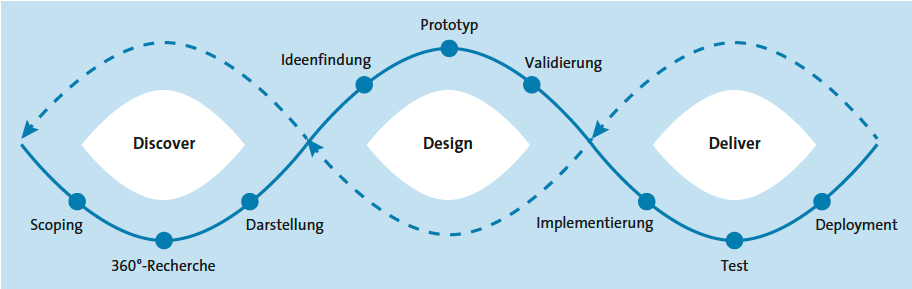
\includegraphics[width=\linewidth]{design_thinking}
  \caption[Phasen des Design-Thinking-Prozesses]{Phasen des Design-Thinking-Prozesses \citep[S. 69]{Elsner2018}}
  \label{}
\end{figure}

\subsection{Aufbau der Arbeit}

\begin{itemize}
  \item Zunächst Industrie 4.0 und treibende Faktoren allgemein
  \item Was ist der Mehrwert von Kommunikationssystemen und welche Protokolle sind Grundlage für die Vernetzung?
  \item Welche Referenzarchitektur vereinheitlicht industrielle Standards und Anforderungen an die Systeme?
  \item Was ist Cloud Computing und welche Rolle spielen dessen Technologien für Industrie 4.0?
  \item Welche Toolsets sind für die Lösung vorhanden?
  \item Use Case: Für welchen Anwendungsfall in der Energiebranche wird ein Prototyp entwickelt?
  \item Was sind die Anforderungen an den Prototypen? Näherer Bezug auf Energiebranche.
  \item Welche Komponenten besitzt das entworfene System bzw. sind notwendig?
  \item Wie sieht die Implementierung im Detail aus?
  \item Evaluierung des Vorgehens
  \item Fazit
\end{itemize}



\newpage


% Insert body
\section{Hauptteil}

% Insert here all subsection as file input
\subsection{Industrie 4.0}
Dieses Kapitel soll die Relevanz der Thematik verdeutlichen, indem sie in einen gesellschaftlichen und wirtschaftlichen sowie in einen technischen Kontext gebracht wird. Zunächst wird erläutert, was hinter dem Begriff \textit{Industrie 4.0} steckt. Dem Ausdruck wird mehr Sinn verliehen, wenn die historische Entwicklung bekannt ist. Anschließend werden die treibenden Technologien kurz erläutert. Da die Venetzung für Industrie 4.0 eine tragende Rolle spielt, werden zuletzt Theorien und Technologien zu Kommunikationssystemen aufgegriffen.
\subsubsection{Definition}

Laut der \cite{FraunhoferGesellschaft2016} habe die \textit{Industrie 4.0} einen revolutionären Einfluss auf die Wertschöpfung in der Industrie und somit auf die Volkswirtschaft. Dieser Marketingbegriff prägt heute die Agenda vieler Unternehmen und Forschungseinrichtungen. Doch was genau hinter dem Begriff zu verstehen ist, bleibt aufgrund des Fehlens einer  \glqq wissenschaftlichen Präzision\grqq{} uneindeutig \citep{Bendel2019}. Für die Gestaltung der digitalen Transformation entstand das Netzwerk \textit{Plattform Industrie 4.0} zwischen der Bundesregierung, Forschungseinrichtungen und Wirtschaft. Dieses hat zum Ziel, die Produktion mittels modernster Informations- und Kommunikationstechnologien entlang der Wertschöpfungkette \glqq flexibler, individueller und effizienter\grqq{} gestalten \citep{BWE2019}. In der Umsetzungstrategie der \citet[S. 8]{BITKOM2015} wird der Begriff wie folgt definiert:

\begin{quotation} \noindent \glqq Der Begriff Industrie 4.0 steht für die vierte industrielle Revolution, einer neuen Stufe der Organisation und Steuerung der gesamten Wertschöpfungskette über den Lebenszyklus von Produkten. Dieser Zyklus orientiert an den zunehmend individualisierten Kundenwünschen und erstreckt sich von der Idee, dem Auftrag über die Entwicklung und Fertigung, die Auslieferung eines Produkts an den Endkunden bis hin zum Recycling einschließlich der damit verbundenen Diensleistungen.\grqq{}
\end{quotation}

Darüber, auf welcher Basis die digitale Transformation in der Industrie stattfinden wird, scheinen sich jedoch alle einig: durch die \textit{intelligente Vernetzung aller am Produktlebenszyklus beteiligten Menschen, Objekte und Systeme} \citep{Roth2016}. Das Wesentliche der Vernetzung bilden dezentrale \acf{cpss} \citep{Bendel2019a}. Die tatsächliche Wertschöpfung ergibt sich aus den in Echtzeit verfügbaren quantitativen Informationen, aus welchen man durch Analysen qualitative Erkenntnisse schließen und optimierte Aktionen auslösen kann \citep{Hnisch2017}. Die  Nach \cite{Sendler2016} gibt es für den Erfolg von \textit{Industrie 4.0} entscheidende Faktoren: Mittlerweile sind digitale Komponenten wie Sensoren, Aktoren oder Kameras so günstig und klein, dass sie in allen möglichen Bereichen eingebaut werden und Umgebungsdaten messen und aufnehmen können. Dank dem Internetprotokoll IPv6 und dem dadurch verfügbaren Adressraum können diese Komponenten ihren Platz im Internet finden. Dass die Informatik sich damit zur wichtigsten Ingenieursdisziplin entwickle, sei unterlässlich, da sie für die Vernetzung der Welt gebraucht werde.

\subsubsection{Historischer Kontext}

Um den aktuellen Stellenwert von Industrie 4.0 zu beschreiben, wird oft von der vierten industriellen \textit{Revolution} gesprochen. Revolutioniert wurde die Industrie erstmalig im 18. Jahrhundert mit der Erfindung der Dampfmaschine durch Thomas Newcomon und James Watt - die \textbf{erste industrielle Revolution} \citep{Roth2016}. Mit Errungenschaften wie dem dampfgetriebenen Webstuhl ging eine \textbf{Mechanisierung }der Produktion einher. Schon damals förderte eine Erfindung, die Lokomotive, eine Vernetzung, die einen regen Warenaustausch ermöglichte \citep{Barthelmaes2017}.

Durch die \textbf{Elektrifizierung} in der Industrie und der Zerlegung von Produktionsschritten in einzelne Einheiten konnten ab 1870 die Waren auf Fließ- und Förderbändern in Massen produziert werden. Angestoßen wurde die \textbf{zweite industrielle Revolution} von Erfindungen wie der Verbrennungskraftmaschine und dem Elektromotor sowie der Herstellung von Syntheseprodukten. Neben fossilen Energieträgern wie Kohle und Öl kam auch die Kernkraft hinzu \citep{Barthelmaes2017}.


Die \textbf{dritte industrielle Revolution} ab den 1970er Jahren, in der wir uns noch heute befinden,  brachte die \textbf{Automatisierung} der Produktion durch die \textbf{Digitalisierung} \citep{Voigt2018}. Getrieben wurde die Revolution durch das Wirtschaftswunder der 1960er Jahre \citep{Roth2016} und ermöglicht durch den Ausbau von Informations- und Kommunikationstechnologien. Entscheidende Technologien waren vielfältig. 1941 entwickelte der Bauingenieur Konrad Zuse den ersten programmgesteuerten und vollautomatischen Computer und setzte den Grundstein für eine rasante Entwicklung der nachfolgenden Technologien. Mit der Vebreitung von Mikroprozessoren, der Miniatisierung der Elektronik sowie der nach dem Mooreschen Gesetz vorausgesagten Zunahme der Prozessorstärke nahm die Welt ein neues Tempo an \citep{Sendler2016}. Einen nicht unwesentlichen Beitrag leistet die Raumfahrtechnik, ohne deren Satellitentechnik eine globale Kommunikation nicht möglich wäre. Da der energieintesive Einsatz dieser Technologien ein Bewusstsein über die Endlichkeit der fossilen Ressourcen schuf, kamen auch erneuerbare Energien hinzu \citep{Barthelmaes2017}.

\begin{figure}[ht]
  \centering
  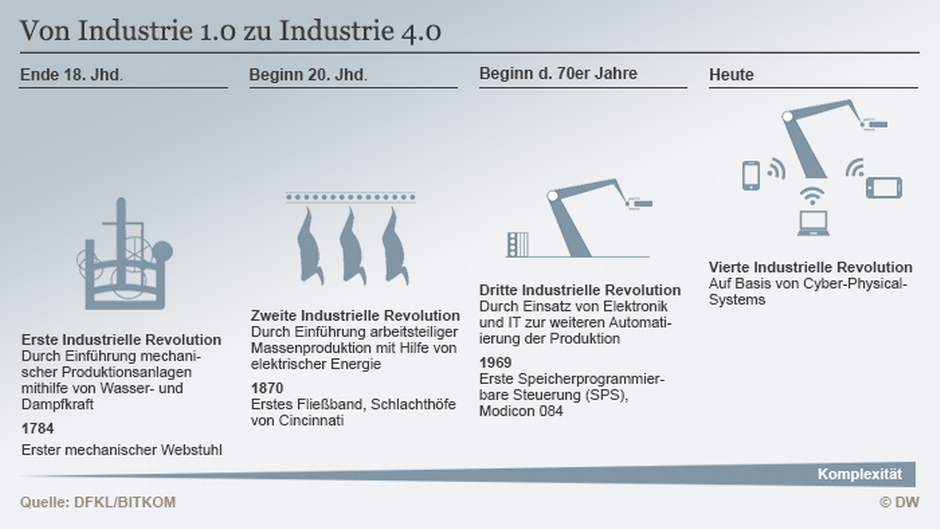
\includegraphics[width=1.0\linewidth]{industrie_40_revolution.png}
  \caption[Die vier Stufen Industrieller Revolutionen]{Die vier Stufen Industrieller Revolutionen\citep{Bauer2015}}
  \label{fig:revolutions}
\end{figure}


Die Industrie 4.0 tatsächlich als \textbf{vierte Industrielle Revolution} zu bezeichnen wird kritisiert, da sie u.a. keine neuen technologischen Innovationen hervorbringe, sondern sich lediglich an den Technologien der dritten Revolution bediene \citep{Barthelmaes2017}. Auch wenn die Technologien nicht unbedingt als revolutionär zu bezeichnen sind, durchlaufen sie eine Evolution und stoßen einen Wandel durch Industrie 4.0 an \citep{Roth2016}. Es entstehen eine Vielzahl neuer Geschäftsmodelle und Produktionsprozesse, die zu Effizienzsteigerungen führen \citep{BITKOM2015}.


\subsubsection{Technologische Treiber}

Industrie 4.0 zeichnet sich durch das Zusammenwachsen der realen und physischen Welt zu mit Sensorik und Aktorik ausgestatten Objekten aus, die per Internet miteinander verbunden sind \citep{BITKOM2015}. Dieses Phänomen ist geprägt von Trendtechnologien wie \textit{Big Data, Internet of Things, Blockchain, Cloud Computing und Machine Learning}, die in kombinierter Nutzung einen Mehrwert erzeugen.
\paragraph{\acf{cpss}}
sind physische Objekte mit einem Datenobekt als virtuelle Präsenz im Netz und bilden die Grundlage von Industrie 4.0 \citep{Drath2016}. Das Hauptmerkmal eines \ac{cpss} ist das mit dem Internet verbundene \textit{eingebettete System}, welches über Sensoren Daten aus der Umwelt aufnimmt, über Aktoren wieder mit ihr interagiert und sich somit an sie anpasst. Diese Fähigkeit, die Informationen zu verarbeiten und zu versenden, wird dem \ac{cpss} durch \textit{Ubiquitous Computing} verliehen. Entscheidend für die implizite und allgegenwärtige Nutzung von IT  ist neben der Austattung mit Sensoren und Aktoren die Verfügbarkeit von Kommunikationsmodulen und Rechenleistung \citep{Roth2016}. Somit wird den Systemen die Fähigkeit verliehen, sich untereinander \textit{dezentral und autonom} zu vernetzen \citep{Bauernhansl2014}. Zudem besitzen \ac{cpss} die Eigenschaft, auch mit Menschen zu interagieren: zum einen über direkte Kommunikation wie Monitoring und Befehle und zum anderen, um komplexe Aufgaben gemeinsam zu lösen \citep{Lueth2016}.


\begin{figure}[ht]
  \centering
  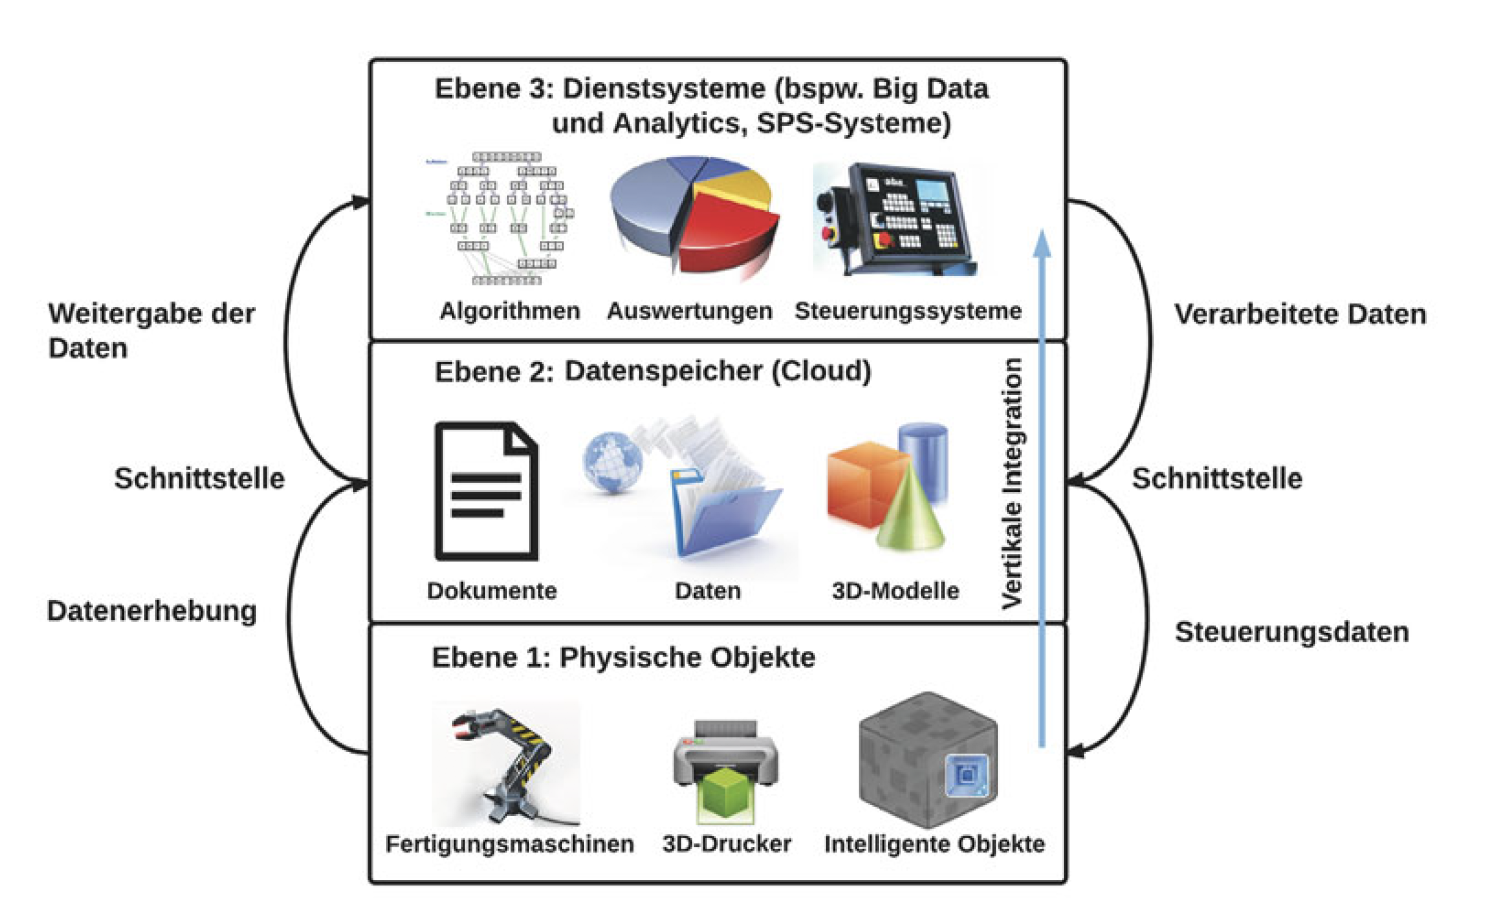
\includegraphics[width=1.0\linewidth]{CPS.png}
  \caption[CPS in der Industrie 4.0]{\ac{cpss} in der Industrie 4.0 \citep[S. 30]{Roth2016}}
  \label{fig:cpskreis}
\end{figure}

\paragraph{Das \acf{iot}} ist das Verbindungsstück zwischen dem Internet und dem Objekt des \textit{Ubiquitous Computing} \citep{Roth2016}. Das Gerät bzw. das \textit{Thing} ist in der Lage dazu, selbstständig den eigenen Zustand zu erfassen und zu kommunizieren \citep{Kenn2016}. Dafür muss das Gerät allerdings eindeutig mit z.B. IP-Adressen oder \ac{rfid} identifizierbar sein. Während das \acf{ipv4} mit seinen rund 4,3 Milliarden Adressen noch nicht einmal die in 2016 verbundenen 6 Milliarden Geräte (siehe Abbildung \ref{fig:connecteddevices}) platzieren kann, schafft das \ac{ipv6} mit 340 Sextillionen (2 hoch 128) Adressen genügend Platz für 20 Milliarden prognostizierte Geräte in 2020. Das Entscheidende für das \textit{Internet} der Dinge ist, dass die Daten nicht lokal auf dem Gerät gespeichert werden, sondern über das Dienste im Internet bestimmten Personen oder Parteien zur Verfügung gestellt werden: \textbf{das Internet der Dinge und Dienste} \citep{Hanisch2017}. Einen Mehrwert bilden die Daten durch die zentrale Aggregation und Analyse, auf deren Grundlage Entscheidungen getroffen werden können. Diese Eigenschaften lassen sich in der für \ac{iot}-Projekte typische Grundarchitektur wiederfinden: \textit{Datentransport, Datenhaltung und Analyse} \citep{Kenn2016}. Der Kreis schließt sich durch die Weitergabe der verarbeiteten Daten als Steuerungsdaten an die Maschine, sodass sich der Fokus von einer Mensch-Maschinen-Interaktion auf eine Maschine-zu-Maschine-Interaktion verschiebt  (s. Abbildung \ref{fig:cpskreis}).

\begin{figure}[ht]
  \centering
  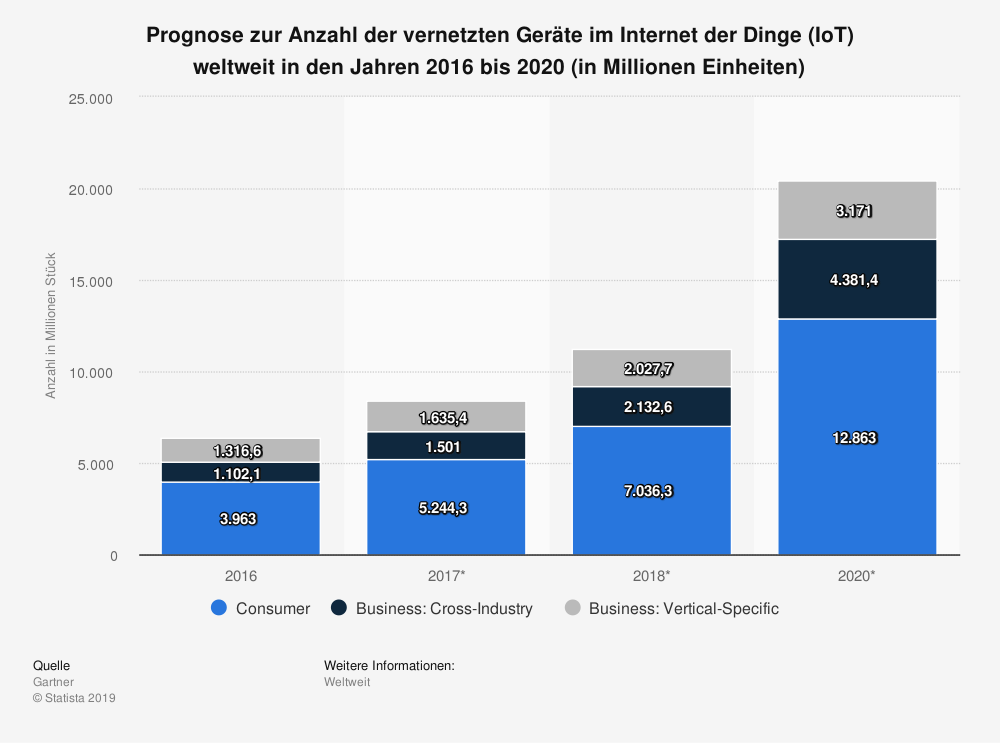
\includegraphics[width=1.0\linewidth]{statistic_connecteddevices.png}
  \caption[Prognose zur Anzahl der vernetzten Geräte im Internet of TThings weltweit]{Prognose zur Anzahl der vernetzten Geräte im \ac{iot} weltweit \citep{Gartner2017a}}\label{fig:connecteddevices}
\end{figure}

\paragraph{Cloud Computing} stellt die IT-Infrastruktur, die ein Industrie 4.0-fähiges \ac{cpss} benötigt. Der \textit{Datentransport} vom Gerät hat oftmals eine Cloud-Plattform als Ziel, auf der die \textit{Datenhaltung} stattfindet \citep{Elsner2018}. Die in die Cloud auslagerbaren Dienste wie Big Data oder Analytics ermöglichen \textit{Analysen} durch Aggregationen und Auswertungen \citep{Roth2016}. Der Nutzen der Cloud steigert sich durch das Kombinieren der Angebote der Cloud-Dienstleister wie Amazon, SAP oder Microsoft \citep{Hnisch2017}. Diese Anbieter stellen besitzen weltweit Rechenzentren, auf denen für Industrie 4.0 ausschlaggebende Services bereitgestellt werden:

\noindent\hspace*{10mm}
 \textbf{Big-Data-Technologien} dienen der Verarbeitung der massiven gesammelten Datenmengen und ermöglichen damit die Nutzung, Verwertung, Vermarktung und vor allem Analyse der digitalen Daten \citep{Radtke2019}.\textcolor{red}{{Wird oft für predictive Maintenance genutzt.}}

 \noindent\hspace*{10mm}
 \textbf{Machine Learning} beruht sich ähnlich wie Big Data auf die \textit{Extraktion von Wissen aus Daten} und ermöglicht dem Computer die selbstständige Ausführung bestimmter Aufgaben, ohne dass sie explizit programmiert werden müssen \citep{Hnisch2017}. Mittels Algorithmen können die Programme aus den Daten lernen und Muster erkennen, aus denen sie Schlussfolgerungen ziehen können \citep{Elsner2018}. Somit könne Aussagen über das wahrscheinlich zukünftige Verhalten des Systems getroffen werden (\textit{Predictive Analytics}), aus denen in Zukunft auch Handlungsoptionen vorgeschlagen werden sollen (\textit{Prescriptive Analytics}) \citep{Huebschle2017}.

 \noindent\hspace*{10mm}
 \textbf{Blockchain} ist die Technologie, auf der die erste Kryptowährung Bitcoin basiert. Die Haupteigenschaften der digitalen Währung sind die Dezentralität sowie  die Unveränderbarkeit und Transparenz der Transaktionshistorie. Auf Grundlage dieser Eigenschaften eines Peer-to-Peer-Systems entwickeln sich neue Geschäftsmodellmuster in verschiedensten Branchen wie Finanzen,  Logistik und Transport, aber auch neue Sicherheitskonzepte \citep{Elsner2018}.

\begin{itemize}
  \item in diesem Kapitel sieht man die Evolution besonders gut
\end{itemize}

\subsubsection{Kommunikationssysteme}

Die Vernetzung ist der Schlüssel zur Dezentralität und Autonomie der \ac{cpss} - und somit zum Erfolg - in der Industrie 4.0 \citep{Bauernhansl2014}. 1980 stellte der Erfinder des Ethernets Robert Meltcafe eine Theorie zum Nutzen eines Netzwerks auf, die mit dem sog. \textit{Netzwerkeffekt} in vielen wissenschaftlichen Disziplinen Anwendungen findet \citep{Lea2018}. Das Konzept besagt,

\begin{quotation}
  \glqq [...] dass der Nutzen eines Kommunikationssystems mit dem Quadrat der Anzahl seiner Teilnehmer wächst.\grqq{} \citep[S. 18]{Bauernhansl2014}
\end{quotation}

Angewandt auf \ac{iot} stellen die Sensoren und Edge-Geräte die Nutzer dar und steigern den Wert der \ac{cpss}, welche die Kommunikationssysteme bilden \citep{Lea2018}. Dem rasanten Anstieg der  miteinander vernetzten Geräte (s. Abbildung \ref{fig:connecteddevices}) liegt außerdem das nach wie vor geltende Moore'sche Gesetz zugrunde \citep{Barthelmaes2017}. Demnach verdoppelt sich die Rechner- bzw. Chipleistung alle zwei Monate bei gleichbleibenden Preisen. Folglich können Technologien, die aktuelle noch zu hohe Preise aufweisen, in Zukunft günstiger betrieben werden \citep{Bauernhansl2014}. Dieser Zusammenhang fördert die Fähigkeiten zur autonomen und intelligenten Vernetzung der dezentralen Systeme und führt zur Effizienzsteigerung \citep{Barthelmaes2017}.
\\\\
Flexibilität in der Vernetzung bieten standardisierte und simple Protokolle wie \ac{rest} und \ac{mqtt} zum Datenaustausch im Internet \citep{Hnisch2017}.

\textbf{\ac{rest}} ist ein Architekturstil, der auf dem \ac{http} basiert und zum Lesen, Erstellen und Bearbeiten von Ressourcen dient. Der Ansatz ist, einheitliche Anfragen an die Ressourcen-Schnittstellen per \ac{uri} zu adressieren und \ac{http}-kodiert zu versenden \citep{Sendler2016}.

\textbf{\ac{mqtt}} ist ein offenes Kommunikationprotokoll, welches zur Übertragung von Telemetriedaten zwischen Maschinen bei niedriger Bandbreite geeignet ist und basiert auf dem Publisher-Subscriber-Prinzip \citep{Lea2018}.
\begin{itemize}
  \item OPCUA
\end{itemize}

\subsection{Digitale Transformation mit Internet of Things}

Eine Umsetzung von Industrie-4.0-Lösungen setzt technische, organisatorische und normative Bedingungen voraus. Während einige Anforderungen für alle Bereiche in der Industrie gelten, unterscheiden sich explizite Anforderungen und Lösungen je nach individuellen Ausgangssituationen von Branchen und Unternehmen \citep{Bauer2014}. Dieses Kapitel soll einen mehrdimensionalen Einstieg in die Thematik der digitalen Transformation bringen. Zuerst wird ein Branchenbezug für die Energiewirtschaft hergestellt. Anschließend folgen allgemeine Herausforderungen zur Umsetzung von IoT-Lösungen für die digitale Transformation. Daraufhin wird eine Referenzarchitektur zur Bewältigung dieser Herausforderungen vorgestellt. Einen wesentlichen Stellenwert in Transformationsprozessen hat das Cloud Computing als technische Voraussetzung, sodass es einer detaillierteren Erläuterung als in \ref{technologien} bedarf. 

\subsubsection{Der Wandel im Energiesektor} \label{energy}

Der Wandel in der gesamten Industrielandschaft von der Mechanisierung und Automatisierung zur Digitalisierung betrifft auf ähnliche Weise auch den Energiesektor. Es gibt in Deutschland kaum eine Branche, die sich innerhalb von zwanzig Jahren so rasant geändert hat wie die Energiewirtschaft \citep{Doleski2015}. Treiber dieser schnellen Entwicklungen sind in erster Linie politisch"=regulatorische Faktoren, welche für darauffolgende Anforderungen die Parameter darstellen.
\\Bis 1998 unterlag die Energieproduktion in Deutschland monopolistischen Strukturen. Wenige Versorgungsunternehmen produzierten in zentralen Werken wie Kernkraftanlagen oder Kohlekraftwerken und schleusten die gewonnene Energie in die Netze ein \citep{Utecht2018}. Die Konsumenten hatten bei der Auswahl ihres Energielieferanten kaum Entscheidungsfreiheit. Mit der Liberalisierung und Privatisierung der Strommärkte öffnete sich jedoch der Binnenmarkt für den Wettbewerb \citep{Doleski2017}. Vor allem durch das \textit{Unbundling}, also der Trennung von Erzeugung und Vertrieb, betraten mehrere Dienstleister für unterstützende Tätigkeiten den Markt. Auch in der Produktion stieg wegen des Wegfalls von Gebietsmonopolen der Trend von zentralen Produktionswerken zu lokalen Erzeugern in der Nähe des Verbrauchers an \citep{Utecht2018}. Grundlegende Veränderungen und Innovationen kamen mit dem Ausbau von erneuerbaren Energiequellen nach der Verabschiedung des Erneuerbare-Energien-Gesetzes von 2000 zur systematischen Förderung von regenerativen Energiequellen. Vor allem nach der Nuklearkatastrophe 2011 in Fukushima wurde die Energiewende stark beschleunigt \citep{Doleski2015}. Der geplante Ausstieg aus Atomkraft und Kohle zwang die Branchen, sich strukturell in der Wertschöpfungskette zu verändern. Die Herausforderung bestand vor allem darin, innerhalb der strengen gesetzlichen Regularien und eines angespannten Finanzrahmens neue Geschäftsfelder zu erschließen \citep{Doleski2015}. So veränderte sich der Produktionstrend von zentraler Erzeugung zu dezentraler Erzeugung mit z.B. Windkraft und Photovoltaik. Die neuen Produktionsmechanismen bedeuten technisch gesehen einen enormen Anstieg der Steuerungskomplexität und eine Belastung der Netzinfrastruktur. Während die Produktion nun vielmehr von schwankenden Umweltbedingungen abhängig ist, bleiben die Anforderungen im Verbrauch, wie die ständige Verfügbarkeit oder die stabile 50-Hz-Netzfrequenz, unverändert \citep{Utecht2018}.
\\\\
\noindent Es sind zwar politisch-regulatorische und ökologische Faktoren, die Umwälzungen in der Energiewirtschaft erzwingen, aber die dezentrale und fluktuierende Energieerzeugung erfordert digitale Lösungen \citep{Doleski2017}. Der Digitalisierung wird eine Schlüsselrolle bei der Lösungsfindung für Dezentralisierung, Flexibilisierung sowie für die effiziente Nutzung von Ressourcen und Energie zugewiesen \citep{FraunhoferISE}. Als \textit{Enabler} für die Energiewende konvergiert die IT-Branche immer mehr mit energiewirtschaftlicher Leistungserstellung \citep{Doleski2015}. Laut dem \citet{BWE2015} wird die Energiebranche eine der ersten voll digitalisierten Branchen der deutschen Volkswirtschaft sein. Zwar kann der Strom nicht digitalisiert werden, aber die Vielzahl von technischen Komponenten in Anlagen müssen sowohl untereinander als auch mit dem Menschen kommunizieren können. Anders als früher ist das gesamte Stromnetz abhängig von einer Vielzahl von Erzeugungsanlagen, die ihren Strom nun in ein intelligentes Stromnetz (Smart Grid) einschleusen müssen. Das Smart Grid kombiniert in einem Netz die Erzeugung, Speicherung und den Verbrauch der Energie. Die dezentralen Erzeugungen werden durch eine zentrale Steuerung aufeinander abgestimmt, sodass Leistungsschwankungen ausgeglichen werden können \citep{Krone2017}. Die Intelligenz wird durch den Datentransport von der Erzeugungsanlage in das Netz gewährleistet. Wenn es zu viele unkoordinierte Anlagen gibt, die ihre Produktionsmengen und ihren Zustand nicht kommunizieren können, kann es zu Instabilität im Netz führen \citep{Umweltbundesamt2018}. Damit die einzelnen Anlagen miteinander kommunizieren können, müssen sie Teil eines \ac{iot}-Netzwerks sein. Somit können sie ihre Umgebungs- und Zustandsdaten eigenständig an ein \acf{cms} senden, das die Daten z.B. in der Cloud sammelt. Für die dort erstellten digitalen Zwillinge der realen Anlagen können auf Grundlage von Analysen der vergangenen und aktuellen Daten prädiktive Wartungsmaßnahmen abgeleitet werden. Daraus kann eine Verbesserung der Qualität und eine höhere Verfügbarkeit des Dienstes resultieren \citep{Utecht2018}.

\begin{figure}[h]
  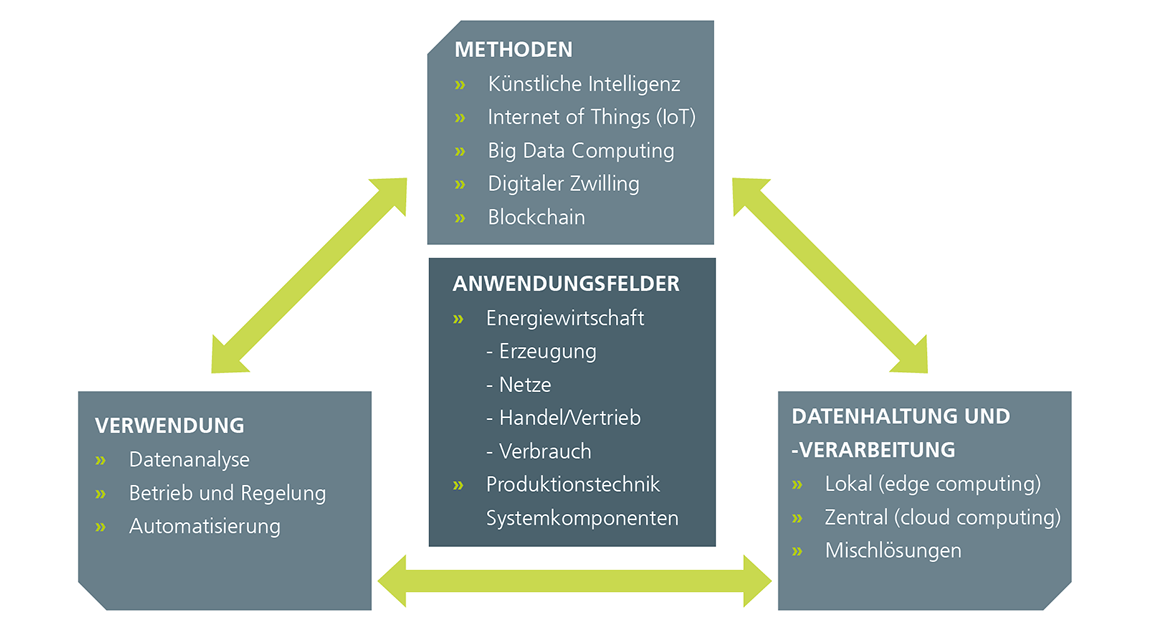
\includegraphics[width=1.0\linewidth]{dimensionen_digitalisierung_fraunhofer.png}
  \caption[Dimensionen der Digitalisierung]{Dimensionen der Digitalisierung \citep{FraunhoferISE}}
  \label{dimensionen}
\end{figure}

\noindent Die rasanten Entwicklungen in den letzten 20 Jahren zeigen, wie wandlungsfähig die Branche ist. Um sich auch zukünftig auf dem Markt bewehren zu können, müssen sich Energieproduzenten und Dienstleister in einem ständigen Anpassungsprozess befinden \citep{Doleski2015}. Essenziell für eine Anpassung an die fortwährende Vernetzung der Produktionswelt ist der Aufbau und die Umsetzung einer unternehmensspezifischen Digitalisierungsstrategie \citep{Koester2017}. Die Herausforderung besteht vor allem darin, die verschiedenen Disziplinen und Dimensionen in der digitalisierten Welt zu berücksichtigen (s. Abbildung \ref{dimensionen}).  Da die Energiebranche besonders gesellschaftlich eine wichtige Rolle innehat, sind die Themen Datenschutz und Sicherheit nicht zu vernachlässigen \citep{Utecht2018}.


\subsubsection{Die Herausforderung IoT}\label{general}

Im Rahmen der Industrie 4.0, die eine Spezialisierung des Internet der Dinge und Dienste darstellt, wachsen die virtuelle und reale Welt zusammen. Daraus ergibt sich die Herausforderung, die Anforderungen der IT, der Elektrotechnik sowie des Maschinenbaus miteinander zu vereinen \citep{Huebner2017}.

\noindent Aufgrund der heterogenen Landschaften und Aussgangssituationen der Unternehmen ist eine Standardisierung der Technologien laut \citet{Bauer2014} unerlässlich. Des weiteren ist die Weiterentwicklung von Breitbandnetzwerken für eine echtzeitfähige Kommunikation von Systemen eine Grundvoraussetzung. Notwendig sind außerdem qualitätsgesicherte Dienste im Internet, die robust gegen Störungen sind. Der Begriff \textit{Internet der Dinge und Dienste} bezieht auf vernetzte Komponenten wie physische Systeme, aber auch auf virtuelle Anwendungen. Da sich die Anzahl und die Beschaffenheit der Applikationen ebenso rasant ändern kann wie die der Geräte, sind eine standardisierte Laufzeitumgebung und Kommunikation für diese von großer Bedeutung. Nicht zu vernachlässigen sind dabei die Sicherheitsaspekte. Die \ac{iot}-Anwendungen bilden eine große Angriffsfläche für Hacker, die durch Sabotage und Manipulation der Systeme eine große Gefahr darstellen. Ein historisches Beispiel für solch eine Gefahr sind die Stuxnet-Angriffe von 2010 auf iranische Atomfabriken \citep{Bauer2014}.

\noindent Allgemein können die Anforderungen und Voraussetzungen für eine \ac{iot}-Lösung auf folgende Begriffe projiziert werden \citep{Acharya2019}:

\begin{itemize}
  \item Skalierbarkeit und Flexibilität
  \item Schnelligkeit
  \item (Ausfall-)Sicherheit
  \item Qualität
\end{itemize}

\subsubsection{Vereinheitlichung durch Referenzarchitektur}\label{rami}

Für die Bewältigung der oben aufgeführten Herausforderungen veröffentlichte die Plattform Industrie 4.0 das \glqq Referenzarchitekturmodell Industrie 4.0\grqq{} (RAMI 4.0) sowie das Konzept zur \glqq Industrie-4.0-Komponente\grqq{}. Beide Modelle wurden 2016 nach DIN SPEC 91345 der Standardisierung zugeführt \citep{Beuth2016}.

\paragraph{RAMI 4.0} ist ein branchenübergreifendes Rahmenwerk, in dem Aufgaben und Abläufe der gesamten Wertschöpfung in überschaubare Teile zerlegt und entsprechenden Normen und Standards zugeordnet werden. Das in Abbildung \ref{rami} dargestellte dreidimensionale Modell ist in Anlehnung auf das Smart Grid Modell erstellt und kapselt die wichtigsten Funktionalitäten aus den verschiedenen Disziplinen in Schichten. Dies schafft Flexibilität für die Konzeptionisierung und Realisierung von Industrie-4.0-Lösungen \citep{Huebner2017}.
\begin{figure}[ht!]
  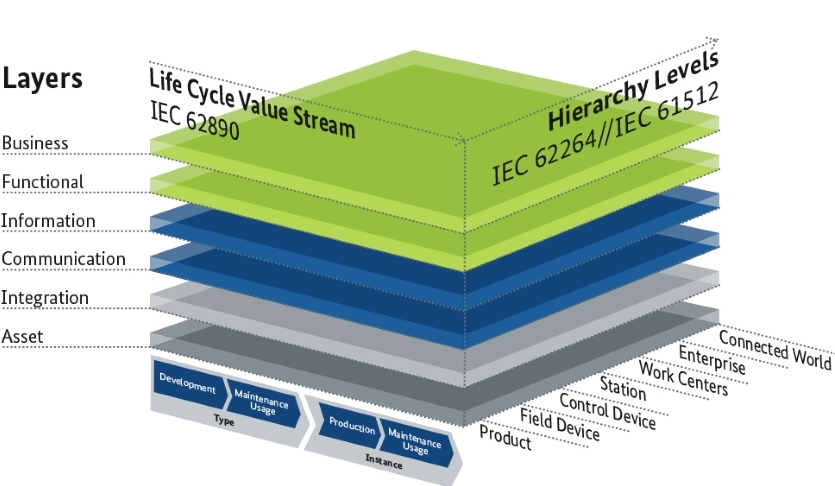
\includegraphics[width=1.0\linewidth]{RAMI.png}
  \caption[Das Referenzarchitekturmodell Industrie 4.0]{Das Referenzarchitekturmodell Industrie 4.0 \citep[S. 42]{BITKOM2015}}
  \label{rami}
\end{figure}
\noindent Für die Migration von Produktionsgegenständen von der heutigen in die Industrie"=4.0"=Welt soll der gesamte Produktlebenszyklus in Daten erfasst und IT"=seitig einheitlich und durchgängig abgebildet werden. Die senkrechte Achse behandelt die IT"=Sicht, die die vertikale Integration der Assets in die Geschäftslogik und deren echtzeitfähige Vernetzung im Produktionsprozess beschreibt. Zu den Assets werden sowohl alle in der Anlage verbauten physischen Komponenten als auch andere Vermögensgegenstände wie Software oder Patente, aber auch Menschen, gezählt \citep{Adolphs2017}. Mit der Ergänzung des Assets um eine \textit{Verwaltungsschale} entsteht die \textit{Industrie-4.0-Komponente}. Die Verwaltungsschale ist das Bindeglied zwischen der realen und der virtuellen Welt. Mit dessen Hilfe wird ein virtuelles Abbild des Assets samt den dazugehörigen Funktionen und Daten erzeugt. Die IT-technische Beschreibung ermöglicht die eindeutige Identifizierung des Assets z.B. durch die \ac{uri}-Adresse im gesamten Wertschöpfungsprozess. Die Aktivitäten für den Übergang in die virtuelle Welt sind in der Integrationsschicht enthalten. Die Dienste zur Steuerung der Integration werden von der Kommunikationsschicht bereitgestellt. Sie dient außerdem der Vereinheitlichung der Kommunikation mit einem durchgängigen Datenformat \citep{BITKOM2015}. Für die Datenkommunikation wird der Standard für industrielle Kommunikation \ac{opcua} empfohlen. Ursache dafür ist zum einen die plattformunabhängige, \ac{soa} und zum anderen die Fähigkeit, die Maschine"=zu"=Maschine"=Kommunikation semantisch zu beschreiben.
\begin{figure}[h]
  \centering
  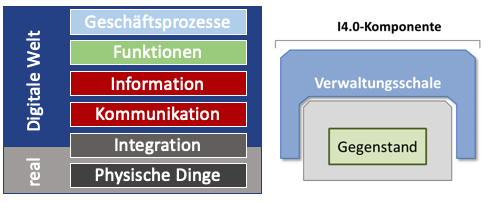
\includegraphics[width=0.7\linewidth]{IT_Sicht.png}
  \caption[IT-Sicht und Industrie-4.0-Komponente]{IT-sicht und Industrie-4.0-Komponente (in Anlehnung an \citet[S. 118]{Adolphs2017}) }
  \label{it_layer}
\end{figure}
Anschließend werden die übertragenen Daten in der Informationsschicht gehalten, wo sie in einer Laufzeitumgebung in einen Regelkontext gebracht werden. Hier werden Regeln für Ereignisse und den Zugriff auf Daten definiert, die in der Funktionsschicht verarbeitet werden. Die tatsächlichen Funktionen eines Assets werden in der Funktionsschicht formal beschrieben. In der funktionalen Schicht befinden sich die Daten in einer Laufzeit- und Modellierungsumgebung für Dienste, die unter anderem Geschäftsprozesse unterstützen. Mit dieser Plattform können die Funktionen horizontal in die Wertschöpfung integriert werden \citep{Huebner2017}. Zusätzlich kann in der Funktionssschicht auf ERP-Funktionen zugegriffen werden. Diese entstehen in der Geschäftsschicht, in der die Modellierung der Regeln für die Geschäftsprozessabwicklung stattfindet. Letztendlich werden die Assets und deren Funktionen hier in die Organisation und Geschäftsprozesse integriert.
\\\\
Jede dieser IT-Schichten liegt an zwei waagerechten Achsen an, welche die horizontale Integration der Produktionsgegenstände in den gesamten Produktionsprozess beschreiben. Die linke Achse soll den gesamten Lebenszyklus von Assets abbilden, während die rechte Achse diese in Hierarchiestufen der Produktions- und Automatisierungstechnik anordnet. Somit können externe Akteure wie Lieferanten oder Kunden, aber auch das erzeugte Produkt in das Industrie-4.0-Netzwerk aufgenommen werden \citep{BITKOM2015}. 

% ************* CLOUD COMPUTING ******************
\subsubsection{Das neue Paradigma: Cloud Computing} \label{cloud}

Flexibilität, Skalierbarkeit, Schnelligkeit, Sicherheit und Qualität präsentieren sich als die wichtigsten Voraussetzungen für die erfolgreiche digitale Transformation eines Unternehmens \citep{Acharya2019}. Für die Erzielung dieser Ziele spielt die in \ref{technologien} bereits kurz erläuterte Cloud eine Schlüsselrolle. Denn die Technologien in der Industrie 4.0 sind zwar nicht neu, aber sie müssen in verschiedenen Kombinationen bei niedrigen Preisen und unabhängig vom Ort stets verfügbar sein. Bei alledem wird dem Nutzer je nach Bedarf das Errichten von IT-Infrastruktur und IT-Ressourcen von dem Cloud-Dienstleister abgenommen \citep{Dzombeta2017}. Entsprechend können die Cloud-Dienste aus folgenden Varianten nach nutzungsbasierten Abrechnungsmodellen wie z.B. dem Pay-Per-Use-Prinzip erworben werden:

\paragraph{\ac{iaas}} Bei dieser Variante stellt das Dienstleistungsunternehmen die notwendige Hardware in virtueller Form zur Verfügung. Es können je nach benötigter Menge Speicherplatz, Prozessorleistung oder Netzkapazitäten bestellt oder wieder abbestellt werden \citep{Dzombeta2017}. Wirtschaftlich bietet das einen großen Vorteil, da die Server von den Anbietern angeschafft, betrieben und gewartet werden, sodass nur die verbrauchte oder vereinbarte Kapazität in Rechnung gestellt wird. Zu den global dominierenden Anbietern gehören Amazon, Microsoft und Google, die in Nordamerika, Europa und Ostasien eine hohe Dichte an Rechenzentren aufweisen \citep{Acharya2019}.

\paragraph{\ac{paas}} Das Dienstleistungsangebot dieser Variante beläuft sich auf die Bereitstellung von Middleware, Laufzeit- und Entwicklungsumgebungen zur Erstellung von Anwendungen, Datenbanken und Webservices. Über definierte Schnittstellen (APIs) kann auf die Entwicklungsumgebung zugegriffen werden \citep{Dzombeta2017}. Da die Plattform auf \ac{iaas} basiert, fällt die Administration von Servern weg \citep{Acharya2019}.

\paragraph{\ac{saas}} Kunden können bei dieser Form meist über Webbrowser auf Software(-pakete) zugreifen, die auf der Infrastruktur des Anbieters gehostet sind. Dabei übernimmt der Anbieter Aufgaben wie Installation, Wartung und Aktualisierung der Software \citep{Utecht2018}. Dieses Prinzip ermöglicht einen schnellen Einsatz sowie eine einfache Austauschbarkeit der Software bei niedrigen Kosten. Aufgrund der Unabhängigkeit von lokalen Installationen kann die Software ortsunabhängig bei verfügbarer Internetverbindung genutzt werden \citep{Dzombeta2017}.

\vspace{0.5cm}
\noindent Die verschiedenen Modelle können auch in Kombination mit dem On-Premise-System genutzt werden.

\noindent Mit diesen Modellen bietet die Cloud einen Raum für die verschiedenen Teilsysteme, die im Industrie"=4.0"=Netzwerk miteinander kommunizieren und Dienste anbieten. Eine \acf{soa} ermöglicht die Interoperabilität der Akteure wie Komponentenhersteller, Automatisierer, Maschinenbauer und Softwarefirmen ohne Master"=Slave"=Beziehungen. In der \ac{soa}-Welt wird nicht mehr zwischen Hard- und Software unterschieden, sodass maschinelle Komponenten ihre Daten genau so als Service zur Verfügung stellen können wie eine Software ihre Funktionen bereitstellt \citep{Adolphs2017}. Entwicklungen wie diese verändern die grundsätzliche Denkweise in der Softwareentwicklung. Alte Architekturen werden von neuen Architekturen wie der \textit{Microservice-Architektur} vertrieben \citep{Acharya2019}.

\begin{figure}[h]
  \centering
  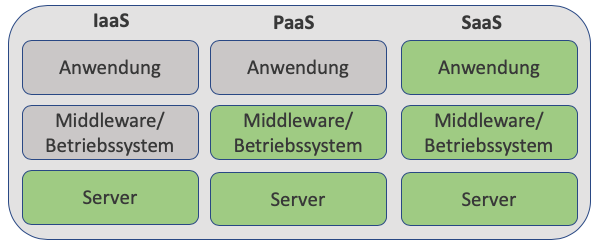
\includegraphics[width=0.8\linewidth]{cloud_variant.png}
  \caption[Die Cloud-Service-Modelle]{Die Cloud-Service-Modelle (In Anlehnung an \citet[S. 88]{Utecht2018})}
  \label{}
\end{figure}

\paragraph{Cloud-native Anwendungen und Microservices}

Die Eigenschaft cloud-nativ besitzen jene Anwendungen, welche in der Cloud \glqq geboren\grqq{} sind und durch Ausschöpfung des Cloud"=Potenzials die Flexibilität, Agilität und Skalierbarkeit von Cloud-Lösungen unterstützen \citep{Acharya2019}. Besonders ist dabei der agile und schnelle Entwicklungsprozess der Software. Eine cloud"=native Anwendung besteht aus mehreren isolierten Services, die unabhängig voneinander entwickelt werden können. Konventionelle Anwendungen sind im Gegensatz dazu monolithischer Natur und basieren meist auf der 3"=Tier"=Architektur. Mit den Bestandteilen Benutzeroberfläche, Datenbank und Anwendungsserver bilden sie ein geschlossenes System. Kleinste Änderungen an einem der Bestandteile führen zu aufwendigen Maßnahmen zur Anpassung des Gesamtsystems \citep{Utecht2018}.
Anders als monolithische Architekturen zeichnet sich die Microservice-Architektur durch ihre einfache und schnelle Erweiterbarkeit und Anpassungsfähigkeit aus. Ein Microservice ist eine spezielle Funktion, oft Geschäftsfunktion, welche in Containern in einer isolierten Umgebung ausgeliefert wird und meist an eine eigene Datenbank angebunden ist. In einer Anwendung kommunizieren diese Microservices über APIs oder Messaging"=Protokolle miteinander und bilden ein Gesamtsystem mit heterogenen Datenquellen. Sollte eine Funktion ein Update erfordern, muss lediglich der Microservice  gewartet werden. Wenn das System eine neue Funktion erfordert, kann ein neuer Microservice einfach hinzugefügt werden, ohne Abhängigkeiten im Gesamtsystem zu stören. Infrastrukturressourcen können bei Bedarf dynamisch zu- oder abgewiesen werden \citep{Acharya2019}.



\subsection{Toolset/Innovationsplattformen}
In den letzten 45 Jahren haben sich die SAP-Technologien durch kontinuierliche Veränderungen an die Anforderungen der digitalen Welt angepasst.
Die Anfänge der Datenverarbeitung von SAP basierte in den 1960er Jahren auf lokalen PCs und der Mainframe-Architektur.
Mit der Client-Server-Architektur und dem darauf basierenden R/3-System konnte die Software ab den 1990er Jahren eine größere
Vernetzung und somit einen größeren Informationsaustausch ermöglichen. Mit der Verbreitung des Internets und dem Ausbau des mobilen
Breitbandnetzes begann zwischen 2000 und 2010 mit den Technologien wie Cloud, Mobile und Big Data eine digitale Transformation \citep[S. 44]{Elsner2018}.
Mit der rasant wachsenden Datenmenge entstanden Möglichkeiten, diese intelligent zu vernetzen und einen Mehrwert daraus zu schöpfen.

\par Im folgenden Kapitel werden ausgewählte Plattformen und deren Eigenschaften beschrieben.
\subsubsection{AWS Cloud}
SNS-Server
Außerdem basiert SCP auf AWS
\subsubsection{SAP Cloud Platform}

SAP Cloud Platform und AWS Microservices und APIs
Programmiersprachen und Laufzeitumgebungen
CF, NEO, ABAP
Destinations

\subsubsection{SAP Leonardo}

Innovationsplattform
GUI, API, SDKs



\newpage

\subsection{Allgemeine Hinweise}
\subsubsection{Querverweise}
Wird in der Arbeit auf andere Stellen (Bilder, Kapitel, Tabellen ...) verwiesen, so ist jeder Verweis immer über Querverweise zu realisieren. In \LaTeX\  sollten dazu z.B. die Befehle $\backslash$ref\{\} und $\backslash$label\{\} verwendet werden.

\subsubsection{Ausdrucke}
Beste Ergebnisse werden erzielt, wenn das Dokument immer auf demselben Drucker in derselben Auslösung ausgedruckt wird. Bei einem Wechsel der Druckertreiber ergeben sich sonst neue Seiten- und Zeilenumbrüche; auch bei einem Wechsel von einem 300dpi auf einen 600dpi Ausdruck entstehen erhebliche Unterschiede im gesamten Dokument. Durch völlig andere Zeilenumbrüche werden Trennungsfehler nicht erkannt; auch das Auffinden von zu korrigierenden Textpassagen wird durch unterschiedliche Ausdrucke erheblich erschwert. Für den endgültigen Ausdruck sind durch diese Abhängigkeit von einem speziellen Druckermodell geeignete Maßnahmen zur Gewährleistung der Verfügbarkeit  der Hardware zu ergreifen.

\subsubsection{Fußnoten}
Fußnoten werden in \LaTeX{} mit dem Befehl $\backslash$footnote\{\} erstellt. Dabei beginnen die einfügten Fußnoten immer mit einem Großbuchstaben und enden mit einem Punkt\footnote{Vergleiche diese Fußnote.}. Fußnoten sind Anmerkungen des Autors vorbehalten, die nicht zwingend zum Verständnis des Haupttextes erforderlich sind (somit im stringenten Argumentationsfluss des Haupttextes stören würden), jedoch für den Leser wertvolle zusätzliche Hinweise enthalten. Es kann sich dabei um Zusatzinformationen (z.B. alternative Formulierungen, Spezifika zitierter Literatur, prägnante Zitate, die im Haupttext stören würden), Erklärungen (z.B. weitere Formelinterpretationen, die jedoch vom Hauptgedankengang ablenken würden) oder Querverweise (Abschnittsverweise in der vorliegenden Arbeit oder spezifische, nicht zitierte Zusatzliteratur) handeln.

\subsubsection{Zitate}
Das Zitieren verwendeter Literatur erfolgt somit nicht in den Fußnoten, sondern im Haupttext unter Verwendung von $\backslash$citep\{\} und $\backslash$citet\{\} sowie BibTeX. Es werden direkte Zitate (d. h. Text wird wörtlich – in Anführungszeichen - übernommen; Quellennachweis ohne ‚vgl.‘) und indirekte Zitate (d. h. sinngemäße Wiedergabe des Textes; Quellennachweis mit ‚vgl.‘) unterschieden. Bei Zitaten mit einer Länge von zwei Seiten wird die erste Seite und "`f."' angegeben, bei mehr als zwei Seiten wird "`ff."' verwendet. 

Zitate werden in \LaTeX{} mit dem Befehl $\backslash$citep\{\} bzw. $\backslash$citet\{\} erstellt. Dabei wird $\backslash$citep\{\} verwendet, um eine Textstelle als Vergleich zu markieren. Hierzu wird vor dem abschließenden Satzzeichen der Befehl $\backslash$citep\{\} eingefügt und mit der entsprechenden Quelle parametrisiert \citep{Example2019}. $\backslash$citet\{\} wird hingegen verwendet, sobald man innerhalb des Fließtexts auf eine Quelle referenzieren will. Dazu fügt man $\backslash$citet\{\} einfach in den Text ein, \glqq so wie es bereits \citet[][]{Example2019} getan haben\grqq.

\subsubsection{Akronyme}
Akronyme werden in \LaTeX{} mit den Befehlen $\backslash$ac\{\}, $\backslash$acf\{\} und $\backslash$acs\{\} erstellt. Zusätzlich muss jedes Akronym definiert werden. Dazu wird in \lstinline{20_lists.tex} eine neue Zeile $\backslash$acro\{\}[]\{\} in der Acronym Umgebung eingefügt. Der erste Parameter beschreibt den Bezeichner für das Akronym über den man später im Text auf das Akronym verweisen kann. Der zweite Parameter stellt das eigentliche Akronym dar und der dritte Parameter ist die ausgeschriebene Langform des Akronyms. Über die drei Befehle $\backslash$ac\{\}, $\backslash$acf\{\} und $\backslash$acs\{\} lassen sich die definierten Akronyme dann im Text verwenden. $\backslash$ac\{\} erzeugt bei erster Verwendung des \ac{acro} die Langform und in Klammern das zugehörige Kürzel, bei jeder weiteren Verwendung erzeugt $\backslash$ac\{\} nur die Kurzform des \ac{acro}. $\backslash$acf\{\} erzwingt die Langform des \acf{acro} auch bei vorheriger Verwendung im Dokument. Äquivalent dazu erzwingt $\backslash$acs\{\} die Kurzform auch wenn das \acs{acro} bisher im Dokument nicht eingeführt wurde.


% Insert conclusion
\section{Schlussteil}
\textcolor{red}{Zum Schluss der Arbeit kann in dem letzten Teil eine thesenartige Zusammenfassung der Untersuchungsergebnisse gegeben werden. Andere Möglichkeiten sind hier auch der Ausblick auf weitere – noch ungelöste – Fragestellungen im Zusammenhang mit dem Thema.}

\subsection{Abschlussbetrachtung}
\textcolor{red}{\blindtext}

\subsection{Reflexion}
\textcolor{red}{\blindtext}



%\pagenumbering{Roman}
%\setcounter{page}{7}

% Insert bibliography
\newpage
\bibliographystyle{apalike}
\bibliography{thesis}

% Insert appendix
\newpage
\appendix

\section{Anhang 1}

\section{Anhang 2}

\newpage


% Insert declaration
\section*{Abschließende Erklärung} \markboth{Erklärung}{}

Ich versichere hiermit, dass ich meine Masterarbeit selbständig und ohne fremde Hilfe angefertigt habe, und dass ich alle von anderen Autoren wörtlich übernommenen Stellen wie auch die sich an die Gedankengänge anderer Autoren eng anlegenden Ausführungen meiner Arbeit besonders gekennzeichnet und die Quellen zitiert habe.

\vspace*{3cm}
\noindent <ORT>, den \today \hspace*{2cm} <AUTOR>


\end{document}
